
\chapter{Human Judgments}
\label{c-human-judgment}

The goal of collecting a human judgment is to get an accurate measurement of  search engine results quality for given set of search tasks. A canonical example is collecting a binary relevance judgment for a document given a TREC-style search topic. The form of human judgment can be quite varied, however, depending on the type of search task and judging target.

We will start with an example to make the discussion more concrete. Figure~\ref{fig:human_judgment_overview} shows a list of possible search tasks about the topic of \textit{crowdsourcing} on the left side, and a few samples from existing web search results for query `crowdsourcing' on the right side.

\emine{Would it be better to show a more standard judging UI here? Like a query and a web page?}
\paul{Can we use another topic? We also discuss crowdsourcing below, which may be confusing. Let's use something which is clearly from a user not a researcher, e.g. ``rules of soccer''. I like the diagram otherwise I think}
\jin{@emine we do show judging I/F later. @paul let's keep it this way unless you strongly disagree -- i've used this topic throughout the chapter so it's not trivial to change}

\begin{figure}
	\begin{center}
		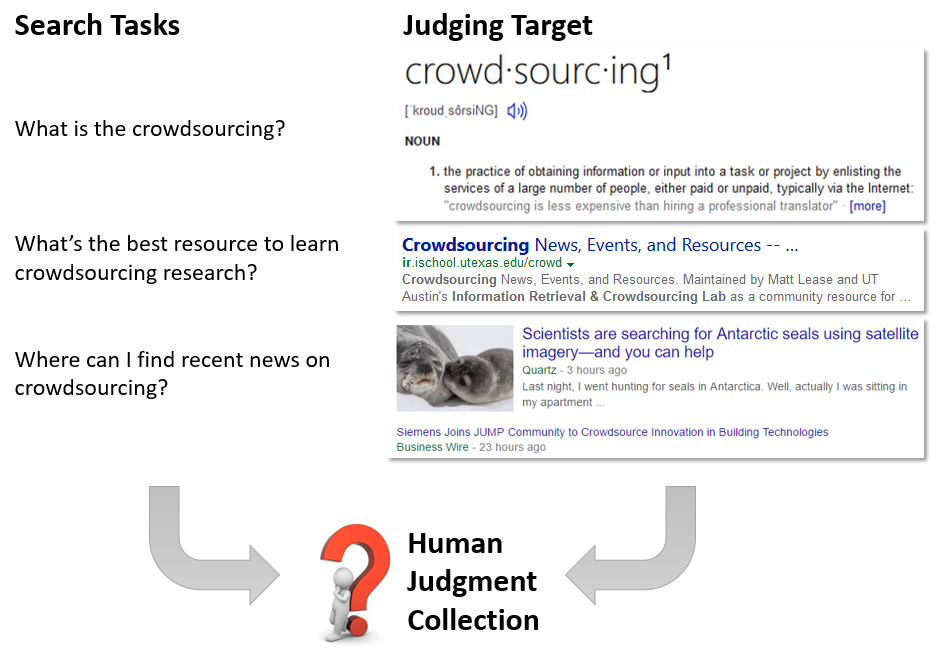
\includegraphics[scale=0.5]{images/human_judgment_overview}
		\caption{Overview of human judgment collection.} 
		\label{fig:human_judgment_overview}
	\end{center}
\end{figure}


This example presents basic ingredients in collecting human judgments -- search tasks and judging targets. From this example one can imagine a myriad of possibilities in designing a human judgment task. You can use either a (potentially ambiguous) keyword query or a well-defined topic description. You can collect judgment for a web document or any SERP element including instant answers or the list of news articles. 

The rest of this chapter is to give you guidance in designing a human judgment, in the light of recent literature on this topic. We will look over how to collect search tasks and how to determine a judging target. Various considerations in designing a judging interface will be examined, as well as the methods for finding and managing human judges.

%The first step in offline evaluation is collecting labels from human judges. In this chapter, we describe various considerations in collecting high-quality labels from human judges at scale. We first discuss the method for collecting search tasks, followed by the design of a judging method. We then discuss the collection of actual judgments, which is an non-trivial task to perform at scale. We also cover the trade-off and in using different types of judging resources -- in-house vs. crowd judges. (20-25 pages)


\section{Collecting Search Tasks}
Before considering judgment design, one needs to collect search tasks on which search results will be evaluated. Search tasks represents users' information needs that needs to be satisfied by the search results. In an industry setting where the search engine is used by actual users, the job of collecting search tasks can be as simple as sampling from queries users issued, whereas without access to such resources one needs to create tasks based on assumptions of target users and information needs. 

\subsection{Creating Search Tasks}
In many cases one needs to perform offline evaluation without a working system -- in building a new product, or in academic setting. It is essential to collect hypothetical search tasks in such cases, which is called simulated search or work (where work includes search and other things) tasks. \cite{Borlund:2003} summarizes the role of simulated work tasks as follows:

% consider non-simulated search tasks?

\begin{quote}
A simulated work task situation, which is a short `cover story', serves two main functions: 1) it triggers and develops a simulated information need by allowing for user interpretations of the situation, leading to cognitively individual information need interpretations as in real life; and 2) it is the platform against which situational relevance is judged. Further, by being the same for all test persons experimental control is provided. Hence, the concept of a simulated work task situation ensures the experiment both realism and control.	
\end{quote}

`Task' can mean different things for different people, and IR literature has long debated over the definition of search task (see \cite{kelly2009methods} for a summary). For our purpose, it is sufficient to understand it as the representation of information needs which a human judge can use to perform a search and\paul{and/or? Often no searching is done by a judge} judge the quality of results.
\emine{Is that the definition of task? May be we should use a more proper definition?}
\paul{task $\neq$ need, but I think this use is blessed by so much past use}

The design of search tasks takes a few considerations which can critically affect evaluation results. First, there is the question of where the task is originated from and how much the judge is interested in or knowledgable about the task, or the corresponding domain. \cite{Edwards:2016} shows that judges' interests in the task has effects on how they perceive and perform the tasks. Judges in general had more knowledge on the tasks they were interested in, expected the tasks to be easier, and had higher engagement in terms of time spent. It is also known that (\cite{Bailey:2008}) judges' knowledge of the domain can affect the quality of the outcome.

Another dimension of task creation is the complexity, which again has many dimensions. \cite{Kelly:2015} looked at this problem using a cognitive complexity framework. They found that participants spent more efforts (queries, clicks and time to completion) in performing tasks with higher cognitive complexity (create, evaluate and analyze) than tasks with lower cognitive complexity (apply, understand, remember).

In sum, these results show that the characteristics of search task is an important dimension in designing an offline evaluation. It is recommended to collect information about task characteristics and design experiments accordingly so that one can control the effect of these factors in evaluation.

%\emine{Should we talk about how to create the tasks?}
%\paul{isn't that what we're doing?}

\subsection{Sampling Query Logs}
Assuming you have a working search engine with real users, it is natural to collect search tasks from query log data. While this is a seemingly straightforward task, there are a few considerations. We outline some below, along with recommendations based on recent studies.

\paragraph{Evaluation Goals} The appropriate sampling strategy depends on evaluation goals. In a typical scenario, it is reasonable to start with a \textit{representative} sample of the traffic \paul{A random sample, you mean? Deduplicated? Balanced/stratified?}. Measurements based on this sampling strategy would lead to the characterization of \textit{average} performance, but there are scenarios where average performance is not informative. 

For example, a recent paper from  \cite{Zaragoza:2010} suggested techniques to identify segments useful for measurement. They introduce the notion of `disruptive sets', which are a set of queries with high quality results in one engine, but not in another. Using a disruptive set, one can focus on the set of queries with a goal to gain competitive advantage.

Other goals can also dictate the choice of sample. For instance, in industry one often targets a specific query segment (e.g., queries with fresh or local search intent); or perhaps on \textit{hard} queries where there is more room for improvement. In these case a sample focusing on the particular segment maximizes the evaluation efficiency.

\paragraph{Characteristics of Search Traffic} The characteristics of search traffic also needs to be considered. \cite{Baeza-Yates:2015} shows that web search query logs follow a power distribution, with longer tails. He suggests a sampling technique to generate a sample that follows this distribution. The main idea is to bin the queries based on the frequency, which allows the sampled queries to match the distribution of original query set. 

\paul{so, stratified and re-balanced?}
\jin{more details?}

\paragraph{Query vs. Task Description} While you can ask judges to imagine a search task given a query, it is open to question whether using query to represent an information need is optimal. Unlike search tasks, which should contain sufficient details of user information need, queries in a typical search engine are often abbreviated in form, often ambiguous and/or with typographical errors \cite{}. \paul{empty cite?}\jin{any recommended citation? i.e., \% of queries with errors}

These characteristics of user queries can be a significant source of noise because 1) there can be many query forms for given information needs, as shown by \cite{Bailey:2015:UVI}, and 2) inferring true information needs from queries can be hard. On the other hand, \cite{Yilmaz:2014:EID} argued that the choice of intent description can also cause large variability in judgment and therefore the judging should be done based on queries.

All in all, despite limitations, user queries are still the most readily available sources of task information, and therefore are widely used for judging search results. One can mitigate the noise and ambiguity of the search query by training judges and presenting possible meanings of the query -- i.e., a SERP from a commercial search engine. We discuss this in detail in Section~\ref{s:judging-context}.

\section{Designing a Judging Interface}

Once the search tasks are collected, we are ready to design a system to gather judgments. There are several main considerations in designing a judging interface: we cover these in what follows.

\begin{enumerate}
	\item  How do we describe the context of a search task? \\(user location, session history, etc.)
	\item  What should be the target of each judgment? \\(webpage, SERP elements or whole SERP)
	\item  What should be the scale of judgment? \\(absolute vs. relative)	
	\item  What is the quality dimension we want to measure? \\(relevance, usefulness, novelty, etc.)
\end{enumerate}

\subsection{Judging Context}
\label{s:judging-context}
There are many contextual variables that affect user satisfaction with any given search result: users' knowledge and preference, language, timing and location of the search, just to name a few. Even with well-defined search tasks, it is hard to specify all these factors, let alone with terse keyword queries. Providing some of this contextual information to judges can potentially reduce the user-judge gap, thereby increasing the judgment quality. \paul{refs?} 

The choice of what context to provide depends again on the evaluation goal -- what do you want judges to be know about the search task? For instance, if you think user location is crucial in judging the relevance of results (which is the case in many tasks), you should present the user's location alongside the query text. Note that, if possible, the location information should be collected along with user queries to get a realistic sample of actual user locations.

Relevance judgments are also affected by what user already did during the session, so it is reasonable to present some part of user session as judging context. Several authors have examined this.\cite{Chandar2013} used a document as context, with the goal of collecting judgments when the context document has already been read. They proposed an evaluation framework for novelty and diversity evaluation. \cite{Golbus:2014:CDR} also experimented with using a document as a context, and found that the metrics based on conditional judgments correlate better with user preference at SERP-level. \paul{other refs?}\jin{on what?}

While one may assume that adding more and more context can only increase the quality of judgments, it should be noted that more context means more effort for judges in digesting and applying the information. Moreover, more context can increase judging cost by adding a further source of variability. That is, instead of collecting judgment for every search task, now that judgments should be collected for every query and context pairs, which can potentially make the evaluation prohibitively expensive. 
\paul{but you just suggested sampling e.g. location at the same time; so there'll be a 1:1 mapping query:context. But it's true that if you want to examine the effect of one more variable (market, location, time, \dots\ then you'll need more data)}\jin{Yes, judging based on query+context will add variance, which necessitates more data}

Therefore, one should carefully consider the value-cost trade-off in adding the context to a judging task. As an extreme example, \cite{Mao:2016} used the entire session as a judging context for collecting judgments on usefulness (as opposed to relevance) and found that usefulness metrics show higher inter-assessor agreement and better correlation with task-level user satisfaction. However, they recommend using usefulness evaluation only for post-hoc analysis of the experiments due to high cost associated with using the whole session as a context.

\subsection{Judging Target}
Judging target defines the basic form of judgment. In what granularity the judgment should be collected (judging unit), and whether the judgment should be given for single item, or a set of items (judgment type). 

\subsubsection{Judging Unit}
Judging unit defines the unit at which judgment should be collected: i.e., in what granularity do we want to collect judgments? In web search, for example, judging unit can be a webpages, SERP elements or a whole SERP, as shown in Figure \ref{fig:judging_units}. 

\begin{figure}
	\begin{center}
		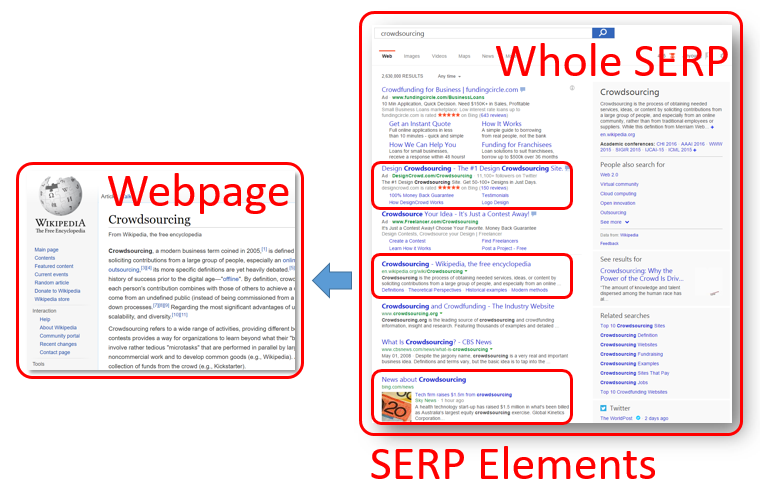
\includegraphics[scale=0.5]{images/judging_units}
		\caption{Various judging units for web search results.} 
		\label{fig:judging_units}
	\end{center}
\end{figure}

Basically, judging unit should be determined by the goal of evaluation: if you care about the quality of ranked list, collecting judgment for each web search result seems like a natural choice. If the presentation of SERP is primary concern, SERP should be the right unit for judgment. 

On the other hand, if the judging target is reasonably complex with multiple sub-components, it is also possible to collect judgments at smaller unit (i.e., SERP elements) and then calculate scores for large unit (i.e., whole SERP) by combining unit scores in a sensible way. This is how most of IR evaluation metrics (i.e., MAP or NDCG) works.

Now, if we want to collect judgment for SERP, should we collect element-wise judgments and then combine, or collect single SERP-level judgment? This question can be generalized into the decision of judging unit when the judging target is complex. In fact, there is no hard and fast rule in determining right judging unit, but here we describe a few trade-offs. 

Smaller judging unit means simpler judging task which can be faster and more reliable individual judging task. However, the number of judgments to evaluate larger judging unit (i.e., SERP) can be quite high if the judging unit is small, making overall judging cost higher than collecting a single judgment for larger judging unit.

Smaller judging unit also means better reusability of individual labels, because you can combine labels for each SERP element to evaluate arbitrary SERP configuration. This means that the cost of collecting judgments can be amortized over multiple experiments. In fact, query-URL relevance judgment has been so widely used in TREC and other settings because it allows the creation of test collection which can be used to evaluate any ranked list.

On the other hand, smaller judging unit makes an assumption that each label can be collected independent of other element. This is hardly true in a typical search scenario where the concept and criteria of relevance can evolve over time. On this regards, larger judging unit has the benefit of providing rich context for judges. Also, larger judging unit can capture the interaction between elements -- i.e., redundancy among documents in a ranked list.

In literature, as briefly mentioned above, document-level judgment is most prevalent. However, there has been a few papers which deal with SERP-level evaluation. \cite{Bailey2010} introduces a judgment scheme which can capture the interaction among SERP elements as well as element-level quality. 

SERP-level judgments were introduced in \cite{Thomas2006}, where they used pairwise judging in order to minimize the complexity of defining judging criteria. (more about this in the following section) Several other works including  \cite{Kim:2013} refined this idea to include dimensional relevance judgments as well as overall SERP-level comparison.
% \cite{Al-Maskari2007} and
\paul{Add work by Falk et al.\ on judging snippets}

\subsubsection{Absolute vs. Relative Judgment}
Another consideration in determining a judging target is the type of judgment, which can be either absolute or relative. In absolute judgment judgment is collected for a single judging target, whereas relative judgment asks for pairwise preference between two judging targets. Figure \ref{fig:judgment_types} shows two types of judgments in evaluating web search results.

\begin{figure}
	\begin{center}
		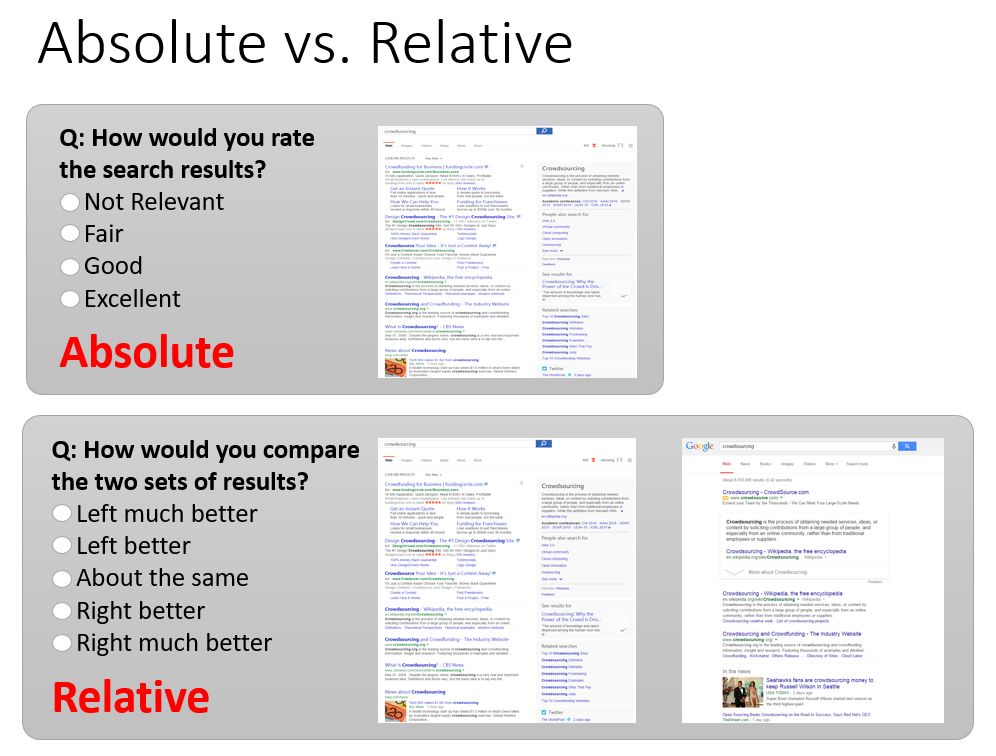
\includegraphics[scale=0.5]{images/judgment_types}
		\caption{Absolute vs. Relative judgments} 
		\label{fig:judgment_types}
	\end{center}
\end{figure}

Now, how should one choose between absolute vs. relative judgment? In general, making an absolute scale judgment requires having objective criteria among different levels, whereas relative judgment can avoid the issue. \cite{CarteretteBCD08} also suggested that relative judgment is more accurate for document-level judging. \cite{Kazai:2013} also found that a pairwise judging mode improves crowdsourcing quality close to that of trained judges.

Relative judgment has been used in various evaluation settings. \cite{Chandar2013} employed document-level pairwise judging using another document as a context, with a goal of novelty and diversity evaluation. \cite{Arguello:2011} also proposed an evaluation scheme for aggregated search based on pairwise preference judgment at element-level. \cite{Zhou:2012} used SERP-level pairwise preference judgment as a part of the evaluation framework for aggregated search.

On the other hand, absolute judgments are reusable in that you can compare among any items for which you have item-level labels, whereas you need to collect labels for every pair of items. Therefore, if you want to reuse judgments in a production environment where multiple generations of ranking techniques should be compared against each other, absolute judgment might save the cost in the long run. This is also the reason that TREC has employed absolute judgment since its inception.
\paul{Add work by Falk et al.\ on magnitude estimation}
\paul{Add work by Diane et al.\ on the effect of question mode? Can't remember if this is relevant}


\subsection{Judging Criteria}
The central assumption of offline evaluation is that human judges can represent real users, and we often want judges to tell us if the judging target would be relevant to the potential user. However, this is not a trivial task for judges given contextual and multi-faceted nature of relevance. (\cite{Borlund:2003}) Actually, \cite{Chouldechova:2013} reports increased judging quality when done by query owners (users who did the search themselves) compared to query non-owners.

Also, while the concept of relevance is broad, it typically specifies the relationship between an information problem and an object, and is not sufficient to capture the true value of the item in the context of search session. Therefore, it has been argued \cite{Belkin:2015:SAL} that IR as a field should move beyond relevance to evaluate usefulness in the context of search task. TREC Session track \cite{carterette2014overview} is another movement in the same spirit.

\jin{Relavance seems to subsume usefulness according to Borlund:2003. But Belkin:2015 seems to use a narrow definition of relevance.}

Recent work have tried to address this problem from multiple angles. The role of user effort and effort-based judging has been proposed \cite{Yilmaz:2014} \cite{VermaYC16}, where it is shown that effort should be incorporated as an additional factor in human judgment to build retrieval systems that optimize user satisfaction. \cite{Golbus:2014:CDR} and \cite{Kim:2013} also experimented with multi-dimensional judgment collection, which is useful in finding the relationship between aspects of relevance.

Another thread of work looked at the relevance judgment in the context of other document, or even the whole session. \cite{Chandar2013} proposed judging methods for novelty and diversity, where they employed preference-based judgment between document A and B in the context of another document (C). The resulting method has benefit of allowing the evaluation of novelty and diversity without requiring the collection of sub-topical judgments. 

\cite{Mao:2016} proposed to collect usefulness judgment in the context of whole session. They showed that high relevance by assessors is a necessary but not sufficient condition for high usefulness for users, and that usefulness judgments better correlates with behavioral signals such as click cumulative gains. But since usefulness judgments are costly to collect, they advised the usefulness judgments for use in post-hoc evaluation.

In overall, current literature suggests many ways to set judging criteria for relevance, with different methods having different emphases. If the goal is to focus on query-document relevance, a simple interface as seen at the top of Figure \ref{fig:judgment_types} will do. However, you can add another document or even whole session history as a context if you want to capture the value of the item in the context of a search task. 

\section{Collecting Judgments}

Once you have judging interface, now you need to find judges to work with. There are quite a few options from which you can find judges, but you can roughly put them into three categories. 1) team members who work on the project 2) expert judges who typically sits in-house with the team 3) crowd judges who work remotely and can be reached via platforms like Amazon Mechanical Turk. 

How should we choose which option to choose? First, it is recommended to start some judging exercise with the team (Group 1) before outsourcing the judging task, because you need to make sure you provide high-quality interface and descriptions to get judgments of reasonable quality. But this approach soon hits scalability issues, so we focus on expert judges (Group 2) and crowd judges (Group 3) in this paper.

There has been a few recent work comparing human judges of different characteristics. \cite{Bailey:2008} is a classic work where they found that judges' level of expertise on the domain can result in small yet consistent difference on system scores and rankings. Similarly, \cite{Chouldechova:2013} looked at judgments done by query owners (users who did the search themselves) vs. query non-owners, where they concluded that query owners are can distinguish a higher quality set of search results from a lower quality set in a blind comparison.

However, neither finding domain experts nor using queries done by judges themselves are feasible if you need judgments at scale, or need to collect judgments from representative sample from traffic. Typically the options available are either in-house judges with some training or crowd judges. Among these groups,  \cite{Kazai:2013} found that trained judges are significantly more likely to agree with each other and with users than crowd workers. But when they compared to judgments with clicks from real users, they found that the judgments from trained judges does not show higher agreement with user clicks.

\subsection{Crowdsourcing Relevance Judgments}

Crowdsourcing has an unparalled benefit in cost and scalability, and it has gathered a lot of attention from research community, and a large body of work has been produced in IR community as well. \cite{Alonso2012} provides an comprehensive survey of research and best practice in this area. 

Since aggregating redundant judgments from a group of independent assessors has been standard approach in reducing errors, some of these work have focused on collecting and aggregating redundant labels. \cite{Venanzi:2014} proposed a community-based Bayesian label aggregation model which is based on finding latent groups among crowd workers and aggregating labels based on them. \cite{Davtyan2015} proposed using textual similar to aggregate crowd judgments, where the relevance labels from similar documents are propagated. Companies such as Crowdflower \footnote{https://www.crowdflower.com/} provide services by which high quality labels are automatically calculated based on redundant judgments.

Another approach in improving the quality of crowdsourced judgments is by improving the judging interface design workflow by which crowd judges work on judging work. This section already dealt with design decisions on judging interface design, and \cite{Kazai2012} provide further guidance in deciding the complexity of judging tasks and the amount of payment per judgment.

Several recent work has investigated workflow design for crowdsourcing. At microscopic level, \cite{Shokouhi:2015} and \cite{Scholer:2013} looked at the effect of previous assessment on the quality of current judgment, where they showed that the human annotators are likely to assign different relevance labels to a document, depending on the quality of the last document they had judged for the same query. At macroscopic level, \cite{Megorskaya2015} explored various parameters in designing workflow, where they argued for having a communication channel between judges and the overlap of 3 -5 for production environment.

\section{Open Issues}

So far in this section, we looked at issues in collecting human judgments, and provided guidances based on latest research. However, the problem of search is rapidly evolving and as such emerging are new areas for research. Before moving on to the next topic, here we discuss several open issues.

\paragraph{New Judging Target} Most of existing research considers document-level judging. But modern SERP contains rich results beyond documents such as instant answers and multimedia results. Extending document-based judging model into these new judging targets would be an interesting problem. This include judging method for captions, instant answers and rich SERPs with all these elements.

\paragraph{New Endpoints for Search} Mobile phone is becoming a standard device for accessing the internet, and recently conversational agent has become a major focus for many tech companies. We still yet to find how this new environment can affect judgment collection. Recent work such as \cite{VermaY16} and \cite{Kiseleva:2016} provide precursor in what needs to change for these new environment.

\paragraph{New Judging Methods} Standard judging methods collect labels given a search task and result pair. However, this model may not work in environments where search is highly contextual and personal. Several recent work such as  \cite{Moraveji:2011} and \cite{Xu:2009} explored task-based judgment collection, where judges perform search given a search engine to make their judgments.
